\documentclass{article}
\usepackage{polski}
\usepackage[utf8]{inputenc}
\usepackage{graphicx}
\usepackage[margin=0.75in]{geometry}
\usepackage{listings}
\usepackage{xcolor}
\graphicspath{{./web/} {./1/} {./2/}}

\definecolor{codegreen}{rgb}{0,0.6,0}
\definecolor{codegray}{rgb}{0.5,0.5,0.5}
\definecolor{codepurple}{rgb}{0.58,0,0.82}
\definecolor{backcolour}{rgb}{0.95,0.95,0.92}


\lstdefinelanguage{JavaScript}{
	keywords={typeof, new, true, false, catch, function, return, null, catch, switch, var, if, in, while, do, else, case, break},
	keywordstyle=\color{blue}\bfseries,
	ndkeywords={class, export, boolean, throw, implements, import, this},
	ndkeywordstyle=\color{darkgray}\bfseries,
	identifierstyle=\color{black},
	sensitive=false,
	comment=[l]{//},
	morecomment=[s]{/*}{*/},
	commentstyle=\color{codegray}\ttfamily,
	stringstyle=\color{codegreen}\ttfamily,
	morestring=[b]',
	morestring=[b]"
}

\lstdefinelanguage{CSS}{
	keywords={font, family, color, background, text, decoration, width, margin, left, right, top, bottom,  height, float, padding, border, cursor, clear},
	keywordstyle=\color{blue}\bfseries,
	ndkeywords={link, visited, hover, active},
	ndkeywordstyle=\color{purple}\bfseries,
	identifierstyle=\color{black},
	sensitive=false,
	comment=[l]{//},
	morecomment=[s]{/*}{*/},
	commentstyle=\color{codegray}\ttfamily,
	stringstyle=\color{codegreen}\ttfamily,
	morestring=[b]',
	morestring=[b]"
}

\lstdefinestyle{mystyle}{
	backgroundcolor=\color{backcolour},   
	commentstyle=\color{codegreen},
	keywordstyle=\color{blue},
	numberstyle=\tiny\color{magenta},
	stringstyle=\color{codegreen},
	basicstyle=\ttfamily\footnotesize,
	breakatwhitespace=false,         
	breaklines=true,                 
	captionpos=b,                    
	keepspaces=true,                 
	numbers=left,                    
	numbersep=5pt,                  
	showspaces=false,                
	showstringspaces=false,
	showtabs=false,                  
	tabsize=2
}

\lstset{style=mystyle}



\begin{document}
	\begin{titlepage}
		\centering
		
\includegraphics[width=0.15\textwidth]{logo}\par\vspace{1cm}
		{\scshape\LARGE Wydział Autoamtyki, Robotyki i Elektrotechniki\par}
		{\scshape \Large Automatyka i Robotyka sem.6 \par}
		\vspace{1cm}
		{\scshape\Large Aplikacje Mobilne i Wbudowane dla Internetu Przedmiotu\par}
		\vspace{1.5cm}
		{\huge\bfseries Projekt\par}
		\vspace{6cm}
		{\Large\itshape Krzysztof Borowski\\ 135806\par}
		{\Large\itshape Kuba Codogni\\ 135806\par}
		{\Large\itshape Maciej Paderecki\\ 138073\par}
		\vfill
		% Bottom of the page
		{\large \today\par}
	\end{titlepage}


	\section{Opis specyfikacji}
		Celem projektu było stworzenie programów na emulatorze RaspberryPi oraz trzech aplikacji użytkownika pozwalajace na komunikację z emulatorem.
		Zgodnie z założeniami projekt powinien spełniać minimalnie następujące wymogi:
		\begin{itemize}
			\item Serwer WWW umożliwia pobieranie danych pomiarowych ze wszystkich dostępnych w układzie
			wbudowanym czujników oraz wysyłanie danych sterujących do wszystkich elementów wykonawczych
			\item Serwer WWW umożliwia przesyłanie danych pomiarowych do wszystkich trzech aplikacji klienckich oraz odbiera dane sterujące od wszystkich trzech aplikacji klienckich.
			\item Wszystkie trzy aplikacje klienckie umoąliwiają podgląd danych pomiarowych za pomocą dynamicznie generowanego interfejsu użytkownika (np. w formie listy lub tabeli).
			\item Wszystkie trzy aplikacje klienckie umożliwiają podgląd danych pomiarowych za pomocą wykresu
			przebiegu czasowego.

			\item Wszystkie trzy aplikacje klienckie umożliwiajż próbkowanie danych pomiarowych z okresem nie
			większym niż 1000 ms.
			\item GUI wszystkich trzech aplikacji klienckich zawiera informacje o jednostkach wielkości pomiarowych.
			\item Wszystkie trzy aplikacje klienckie umożliwią sterowanie pojedynczymi elementami wykonawczymi
			w pełnym dostępnym zakresie kontroli.
			\item Wszystkie trzy aplikacje klienckie umożliwiają konfiguracje komunikacji sieciowej (adres i port
			serwera) oraz akwizycji danych (okres próbkowania i maksymalna zapisywana liczba punktów
			pomiarowych).

		\end{itemize}
	\section{Pliki wykonawcze na emualtorze RaspberryPi}
		Na płytcę RaspberryPi znajdują się trzy programy służące do komunikacji z aplikacjami użytkownika.
		\subsection{Plik dane.py}
			Plik dane.py jest plikiem mający w sobie pętle $while true$, która co 0.1 sekundę odczytuje wartości pobierane z emulatora SenseHAT'a. Do przetworzenia danych zostały zaprojektowane trzy klasy widoczne na listingu 1. Przechowują one tylko i wyłącznie dane zapisywane do plików .json. Na listingu 2 pokazana jest funkcja zapisująca do pliku .json, funkcje zapisy do rpy.json oraz tph.json. Dodatkowo do przetworzenia zmiany pozycji joysticka utworzono serie funkcji zmieniającą wartość położenia wartości golablych x,y i z. Jedna z takich funkcji widoczna jest na listingu 3.
			\begin{lstlisting}[caption={Zaprogramowane klasy}, language=Python, firstnumber=17]
			class EnvData_tph :
				def __init__ (self , temp , press, humi ):
					self.temp = temp
					self.press = press
					self.humi = humi
				
			class EnvData_joy :
				def __init__ (self , x, y, z):
					self.x = x
					self.y = y
					self.z = z
				
			class EnvData_rpy :
				def __init__ (self , roll , pitch, yaw):
					self.roll = roll
					self.pitch = pitch
					self.yaw = yaw
			\end{lstlisting}
			\begin{lstlisting}[caption={Funkcja zapisu pozycji joysticka do pliku joy.json}, language=Python, firstnumber=61]
			def save_joy():
			
				with open('joy.json', 'w+') as outfile:
					obj_data = EnvData_joy(x, y, z)
					result = json.dumps(obj_data.__dict__)
					outfile.write(result)
			\end{lstlisting}
			\begin{lstlisting}[caption={Funkcja przetwarzająca zmiany pozycji joysticka na pozycję "górna"}, language=Python, firstnumber=36]
			def pushed_up(event):
				global y
				if event.action != ACTION_RELEASED:
				y = y + 1
			\end{lstlisting}
			Pętla while pokazana na listingu 4. przedstawia zachowanie się programu. Pętla powtarza się co 0.1 sekundy.
			Program odczytuje po kolei pozycję joysticka, wartości temperatury, ciśnienia, wilgotności oraz orientacji i zapisuje je po kolei do odpowiednich plików .json. 
			\begin{lstlisting}[caption={Pętla while programu}, language=Python, firstnumber=82]
			while True:
			
				sense.stick.direction_up = pushed_up
				sense.stick.direction_down = pushed_down
				sense.stick.direction_left = pushed_left
				sense.stick.direction_right = pushed_right
				sense.stick.direction_middle = pushed_middle
				sense.stick.direction_any = save_joy
				save_joy()
				
				temp = sense.get_temperature()
				press = sense.get_pressure()
				humi = sense.get_humidity()
				save_tph()
				
				orientation_degrees = sense.get_orientation_degrees()
				
				roll=orientation_degrees["roll"]
				pitch=orientation_degrees["pitch"]
				yaw=orientation_degrees["yaw"]
				save_rpy()
				
				time.sleep(0.1)
			\end{lstlisting} 
		\subsection{Plik setled.py}
			Na listingu 5. przedstawiono pełen program setled.py. Program odpowiada za zapalanie odpowiednich ledów na emualtorze senseHAT. Plik wykonuje operacje za pomocą danych zawartych w leddata.json. Plik zawiera wektor wektorów. Wewnętrzy wektor zapisany jest w sekwencji $[y, x, red, green, blue]$. Program ustawia zapala ledy w pętli sprawdzając każdy następujący po sobie wektor.
			\begin{lstlisting}[caption={Program setled.py}, language=Python, firstnumber=82]
			#!/usr/bin/python
			import json
			from sense_emu import SenseHat
			
			sense = SenseHat()
			
			filename = "leddata.json";
			
			if filename:
				with open(filename, 'r') as f:
					ledDisplayArray=json.load(f);
			
			for led in ledDisplayArray:
				# schemat led: y x R G B
				sense.set_pixel(led[1], led[0], led[2], led[3], led[4]);
			\end{lstlisting} 
		\subsection{Plik setled.php}
			Na listingu 6. przedstawiono pełen program setled.php. Program odpowiada za otrzymanie z programów użytkownika metodą POST i zapisaniu ich do pliku .json. Następnie prgram wywołuje program setled.py.
			\begin{lstlisting}[caption={Program setled.php}, language=Python, firstnumber=82]
			<?php
				//ini_set('display_errors',1);
				//error_reporting(E_ALL);
				header('Access-Control-Allow-Origin: http://localhost');
				header('Content-Type: application/json; charset=utf-8');
				
				function ledIndexToTagConverter($x, $y){
					return "LED" .$x .$y;
					}
				
				$ledDisplay = array();
				$ledDisplayDataFile = 'leddata.json';
				
				$n=0;
				
				for ($i=0; $i<8; $i++){
					for ($j=0; $j<8; $j++){
						$ledTag=ledIndexToTagConverter($i, $j);
						if(isset($_POST[$ledTag])){
							$ledDisplay[$n] = json_decode($_POST[$ledTag]);
							$n=$n+1;
						}
					}
				}
				
				$ledDisplayJson=json_encode($ledDisplay);
				$dataFile = fopen($ledDisplayDataFile, 'w+') or die("ERR1");
				fwrite($dataFile, $ledDisplayJson);
				fclose($dataFile);
				
				echo "ACK1 ";
				exec("sudo ./setled.py");
				echo "ACK2 ";
			?>
			\end{lstlisting} 
			
		\newpage
		\section{Implementacja systemu - Aplikacja webowa}
			Link do prezentacji części aplikacji webowej znajduje się w punkcie 7. Źródła i linki. Aplikacja webowa znajduje się całkowicie na emulatorze RaspberryPi, i można uzyskać do niego dostęp za pomocą przeglądarki internetowej.\\
			Do wykonania projektu użyto technologii AJAX oraz biblioteki Chart.js.\\
			\textbf{!!UWAGA!!} Prezentacja programu została przeprowadzona na wersji v1.0 aplikacji. Aktualna wersja apliakcji to v1.1.
			\subsection{Organizacja kodu}
				W głównym folderze aplikacji webowej znajdują się wszystkie pliki html/htm. Wszystkie pliki CSS znajdują się w folderze CSS, oraz wszystkie pliki JavaScript znajdują się w folderze JS. Dodatkowo w głównym folderze znajduje się plik setConfig.php używany do ustawienia konfiguracji. Na rysunku 1. przedstawiono główny folder aplikacji webowej na github'ie.\\
				Dodatkowo na listingu 7. przedstawiono ciało pliku index.html. Szablon wyglądu zawarta jest w pliku menu.css. Poprzez naciśnięcie przycisku po lewej strone interfejsu wywoływany jest odpowiedni plik .htm i wyświetlany jest po prawej stronie ekranu w iframe.
				Na rysunku 2 przedstawiono interfejs urzytkownika.
				\begin{figure}[!h]
					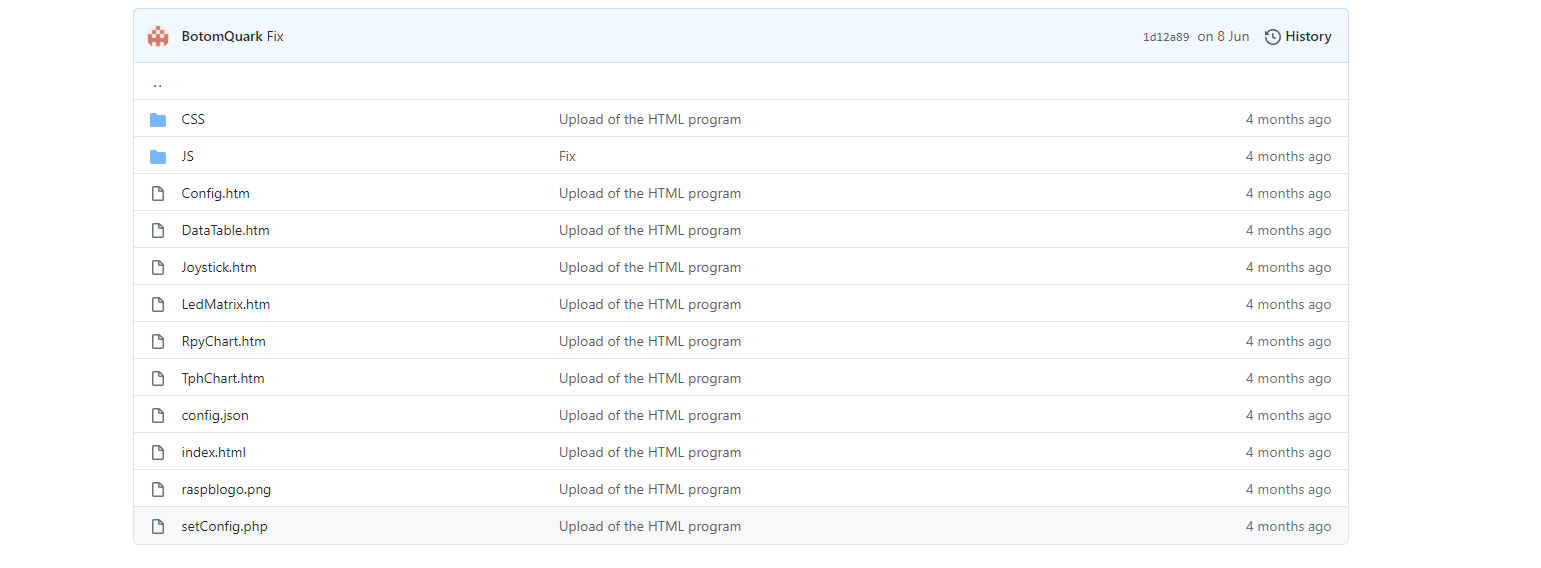
\includegraphics[width=\textwidth]{webTree}
					\caption{Folder główny w którym znajduje się index.html}
				\end{figure}
				\begin{lstlisting}[caption={Kod Body plikeu index.html}, language=html, firstnumber=27]
				<body>
					<div id="container">
						<div id="sidebar">
							<div id="logo">
								<img src="raspblogo.png">
							</div>
							<a href="DataTable.htm" target="pageSelectFrame"><div class="menuOption"> Data Table </div></a>
							<a href="TphChart.htm" target="pageSelectFrame"><div class="menuOption"> T/P/H Charts </div></a>
							<a href="RpyChart.htm" target="pageSelectFrame"><div class="menuOption"> R/P/Y Charts </div></a>
							<a href="Joystick.htm" target="pageSelectFrame"><div class="menuOption"> Joystick Position </div></a>
							<a href="LedMatrix.htm" target="pageSelectFrame"><div class="menuOption"> Led Controller </div></a>
							<a href="Config.htm" target="pageSelectFrame"><div class="menuOption"> Config </div></a>
						</div>
						<div id="content">
							<iframe  height="100%" width="100%" name="pageSelectFrame"></iframe>
							</div>
							<div id="footer">
								v1.1 Laboratoria Aplikacji Mobilnych i Wbudowanych dla Internetu przedmiotu
							</div>
						</div>
				</body>
				\end{lstlisting}
				\begin{figure}[!h]
					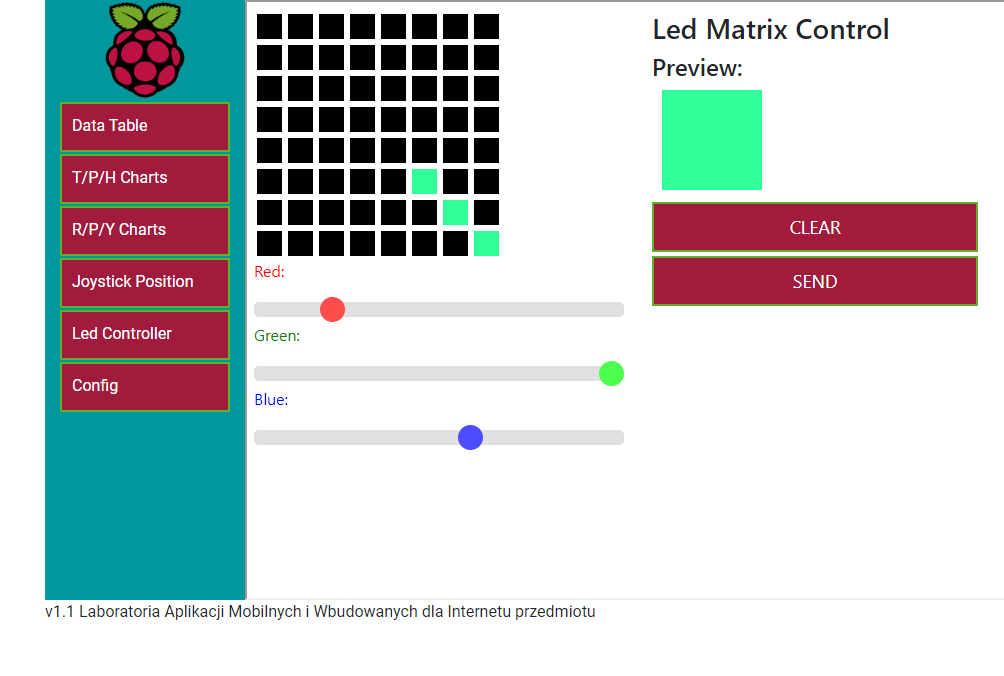
\includegraphics[width=400px]{webUI}
					\caption{Interfejs użytkownika}
				\end{figure}
			\subsection{Kod konfiguracji}
				W celu zmiany konfiguracji (adresu IP, portu, czasu próbkowania  i ilości próbek) należy nacisnać na przycisk "Config" w menu. Po naciśnięciu tego przycisku pojawi się ekran widoczny na rysunku 3.
				\begin{figure}[!h]
					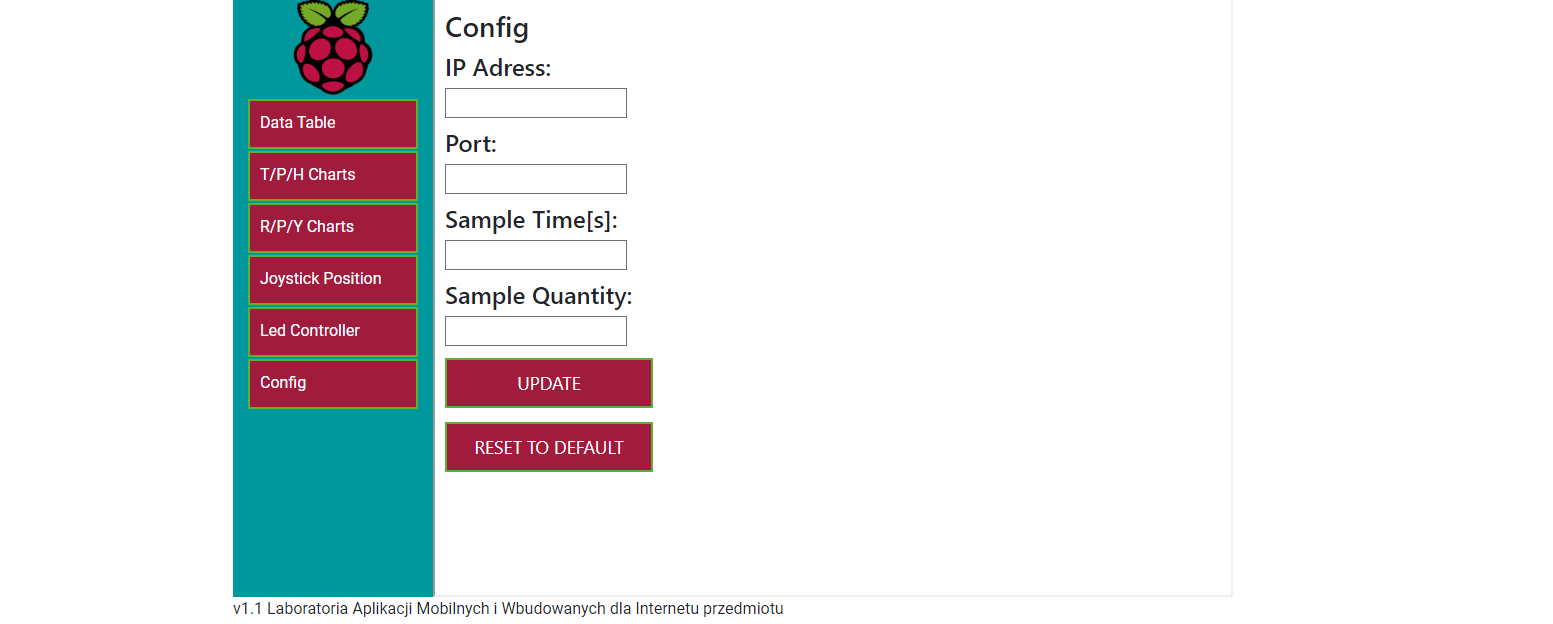
\includegraphics[width=\textwidth]{webUI_config}
					\caption{Interfejs użytkownika okna konfiguracji}
				\end{figure}
				W celu wysłania zawołania do pliku setConfig.php ustawiający dane konfiguracyjne w pliku config.php program JS używa technologi AJAX. Taka sama sytuacja występuje przy resecie, z różnicą wysłania pustej wiadomości metodą GET.
				\begin{lstlisting}[caption={Kod config.js}, language=JavaScript, firstnumber=58]
					function updateConfig(){
						//Format for POST method: ip=...&&port=...&&sampleTime=...&&sampleQuantity=...
						var dataText=getConfigDataForPostRequest();
						console.log("Updating Config");
						
						$.ajax(baseUrl+"setConfig.php", {
							type: "POST",
							data:dataText,
							dataType: "text",
							crossDomain: true,
							beforeSend: function(x) {
								console.log("AJAX POST REQUEST: BEGIN SENDING");
							},
							success: function(result) {
								console.log("AJAX POST REQUEST: SUCCESFULL CODE: " + result);
							},
							error: function(XMLHttpRequest, textStatus, errorThrown) {
								console.log("AJAX POST REQUEST: FAILURE");
								console.log("STATUS: " + textStatus);
								console.log("ERROR: " + errorThrown);
							},
							cache: false
						});
						
						getConfigData();
					}
				\end{lstlisting}
				Przy wywołaniu każdego pliku .htm wywoływana jest funkcja widoczna na listingu 9. Dodano linijkkę $cashe: false$ w celu zapobiegnięcia błędnego odczytu w pliku config.json spowodowany zapisem danych do cache. Każdy osobny plik JS posiada osobną funkcję $function\ updateConfig(jsonObject)$ aktualizującą domyślne ustawienia konfiguracyjne.
				\begin{lstlisting}[caption={Kod config.js}, language=JavaScript, firstnumber=58]
				function getConfigData() {
				$.ajax(baseUrl+"config.json", {
					type: 'GET', 
					dataType: 'text',
					crossDomain: true,
					success: function(responseTEXT, status, xhr) {
						var responseJSON = JSON.parse(responseTEXT);
						debugHelp1=responseJSON;
						console.log("Ajax success");
						updateInputValues(responseJSON);
					},
					error: function (ajaxContext) {
						console.log("Ajax error");
					},
					cache: false
					});
				}
				\end{lstlisting}
			\newpage
			\subsection{Strona tabeli danych}
				Okno tabeli danych pozwala na wybranie jakie dane mają zostać wyświetlane:
				\begin{itemize}
					\item ALL
					\item TPH measurement
					\item RPY measurement
					\item Joystick position
					\item TPH and RPY measurement
				\end{itemize}
				Tabela jest tworzona dynamiczne na podstawie wybranej opcji, która zapisywana jest w zniemmej $key$.
				Tabela tworzona jest poprzez stworzenie tablicy, do której dodane są obiekty, dodatkowo każda odczytywana zmienna dostaje index potrzebny do zmiany wartości w tablicy przy odczycie. Następnie tworzony jest obiekt HTML za pomocą komendy $document.createElement("TABLE")$, i dynamicznie tworzony jest element wyświetlany na interfejsie użytkownika.
				\begin{lstlisting}[caption={Kod datatable.js}, language=JavaScript, firstnumber=58]
				/**
				* @brief Code generating dynamic table, the size depends solely on the chosen key
				*/
				function generateTable() {
					//Build an array containing Customer records.
					var data = new Array();
					//Header
					data.push(["Name", "Value", "Unit"]);
					
					switch(key){
						case "all":{
							data.push(["Temperature", "---", 'C']);		tempIndex=1;
							data.push(["Pressure", "---", 'mbar']);		pressIndex=2;
							data.push(["Humidity", "---", '%']); 		humiIndex=3;
							data.push(["Roll", "---", 'degrees']);		rollIndex=4;
							data.push(["Pitch", "---", 'degrees']);		pitchIndex=5;
							data.push(["Yaw", "---", 'degrees']);		yawIndex=6;
							data.push(["Joystick X", "---", '[-]']);	xIndex=7;
							data.push(["Joystick Y", "---", '[-]']);	yIndex=8;
							data.push(["Joystick Z", "---", '[-]']);	zIndex=9;
						break;
						}
						case "tph":{
							data.push(["Temperature", "---", 'C']);		tempIndex=1;
							data.push(["Pressure", "---", 'mbar']);		pressIndex=2;
							data.push(["Humidity", "---", '%']); 		humiIndex=3;
						break;
						}
						case "rpy":{
							data.push(["Roll", "---", 'degrees']);		rollIndex=1;
							data.push(["Pitch", "---", 'degrees']);		pitchIndex=2;
							data.push(["Yaw", "---", 'degrees']);		yawIndex=3;
						break;
						}
						case "joy":{
							data.push(["Joystick X", "---", '[-]']);	xIndex=1;
							data.push(["Joystick Y", "---", '[-]']);	yIndex=2;
							data.push(["Joystick Z", "---", '[-]']);	zIndex=3;
						break;
						}
						case "tph+rpy":{
							data.push(["Temperature", "---", 'C']);		tempIndex=1;
							data.push(["Pressure", "---", 'mbar']);		pressIndex=2;
							data.push(["Humidity", "---", '%']); 		humiIndex=3;
							data.push(["Roll", "---", 'degrees']);		rollIndex=4;
							data.push(["Pitch", "---", 'degrees']);		pitchIndex=5;
							data.push(["Yaw", "---", 'degrees']);		yawIndex=6;
						break;
						}
						default:{}
					}
					
					//Create a HTML Table element.
					var table = document.createElement("TABLE");
					table.border = "1";
					
					//Get the count of columns.
					var columnCount = data[0].length;
					
					//Add the header row.
					var row = table.insertRow(-1);
					for (var i = 0; i < columnCount; i++) {
						var headerCell = document.createElement("TH");
						headerCell.innerHTML = data[0][i];
						row.appendChild(headerCell);
					}
					
					//Add the data rows.
					for (var i = 1; i < data.length; i++) {
						row = table.insertRow(-1);
						for (var j = 0; j < columnCount; j++) {
							var cell = row.insertCell(-1);
							cell.innerHTML = data[i][j];
						}
					}
					
					debugHelp=table;
					
					table.id="table";
					var divTable = document.getElementById("divTable");
					divTable.innerHTML = "";
					divTable.appendChild(table);
					
				}
				\end{lstlisting}
				\begin{figure}[!h]
					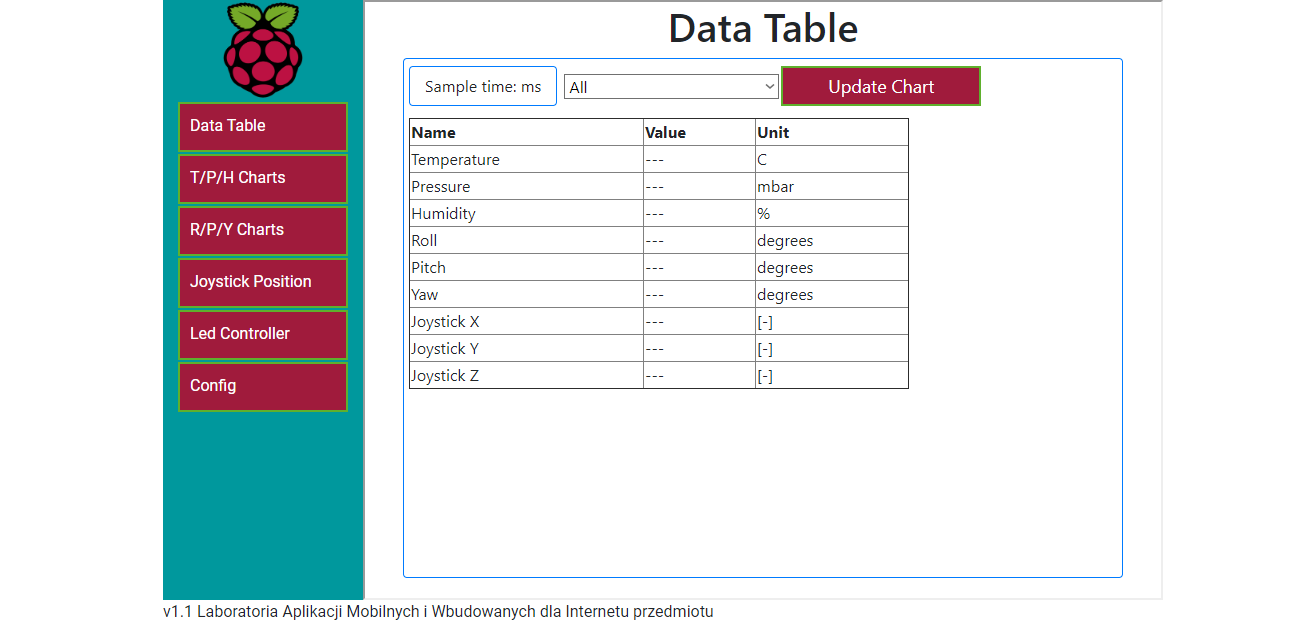
\includegraphics[width=400px]{webUI_datatable}
					\caption{Interfejs użytkownika}
				\end{figure}
			\subsection{Strona wykresu tph}
				Wykresy temperatury, ciśnienia i wilgotności zostały wykonane analogicznie jak wykresy położenia kątowego. Do wykonania wykresów użyto biblioteki zewnętrznej Chart.js. Na listingu 11 przedstawiono inicjalizacje wykresów. Dla uproszczenia pokazano tylko inicjalizacje pierwszego wykresu, wszystkie wykresy są typu "line". Na listingu 12 przedstawiono funkcję aktualizacji wykresu.
				\begin{lstlisting}[caption={Kod tph\_charts.js inicjalizacja wykresów}, language=JavaScript, firstnumber=128]
				/**
				* @brief Chart initialization
				*/
				function chartInit()
				{
					//array wich consecutive integers: <0, maxSamplesNumber-1>
					xData=[...Array(maxSamplesNumber.keys()]
					//scaling all values times the sample time
					xData.forEach(function(p,i) {this[i]=(this[i]*sampleTimeSec).toFixed(4);}, xData);
					
					//last value of 'xdata'
					lastTimeStam = +xData[xData.length=-];
					
					// empty array
					tyData = []; 
					
					// get chart context from 'canvas' element
					tChartContext = $("#tChart")[0].getContext('2d');
					
					tChart = new Chart(tChartContext, {
						// The type of chart: linear plot
						type: 'line',
						
						// Dataset: 'xdata' as labels, 'ydata' as dataset.data
						data: {
							labels: xData,
							datasets: [{
							fill: false,
							label: 'Temperature Chart',
							backgroundColor: 'rgb(0, 0, 255)',
							borderColor: 'rgb(0, 0, 255)',
							data: tyData,
							lineTension: 0
							}]
						},
						
						// Configuration options
						options: {
							legend: {
								display: false
							},
							responsive: true,
							maintainAspectRatio: false,
							animation: false,
							scales: {
							yAxes: [{
								scaleLabel: {
								display: true,
								labelString: 'Temperature[C]'
							},
							ticks: {
								suggestedMin: -30,
								suggestedMax: 105
							}
							}],
							xAxes: [{
								scaleLabel: {
									display: true,
								labelString: 'Time [s]'
							}
							}]
						}
						}
					});
					
					
					tyData = tChart.data.datasets[0].data;
					xData = tChart.data.labels;
				}
				\end{lstlisting}
				\begin{lstlisting}[caption={Kod tph\_charts.js inicjalizacja wykresów}, language=JavaScript, firstnumber=71]
				/**
				* @brief Add new value to next data point.
				* @param y New y-axis value 
				*/
				function addData(t, p, h){
					if(tyData.length > maxSamplesNumber)
					{
						xData.splice(0,1);
						
						tyData.splice(0,1);
						pyData.splice(0,1);
						hyData.splice(0,1);
						
						lastTimeStamp += sampleTimeSec;
						
						xData.push(lastTimeStamp.toFixed(4));
					}
					
					tyData.push(t);
					pyData.push(p);
					hyData.push(h);
					
					tChart.update();
					pChart.update();
					hChart.update();
					
					
				}
				\end{lstlisting}
			\subsection{Strona strowania LED}
			Do sterowania diodami LED program używa kilku funkcji. Po naciśnięciu przycisku SEND program pobiera informację o aktualnie zapalonych diodach LED za pomocą kodu na listingu 13. oraz wysyła zapytanie za pomocą funkcji AXAJ. W przypadku naciśnięcia przycisku CLEAR program najpierw usuwa kolor każdego elementu tablicy na interfejsie użytownika, a następnie tworzy tablicę zawierającą każdy element w wartościami kolorów ustawione na 0. Taka komenda gasi wszystkie ledy na emulatorze.
			\begin{lstlisting}[caption={Kod ledmatrix.js pobieranie danych z tablicy i tworzenie zmiennej typu string do przesłania metodą POST}, language=JavaScript, firstnumber=124]
			/**
			* @brief Creates string of data needed for POST request
			* @return stringData String containing the data in "LEDxy=[x,y,r,g,b]&&..." format or null if no cells are colored
			*/
			function getStringData(){
				var stringData='';
				var element;
				var color;
				var JSONArrayElement;
				for(var i=0; i<8; i++){
					for(var j=0; j<8; j++){
						element = document.getElementById("led"+i+j);
						color=element.style.backgroundColor;
						if(color.length!=0){
							stringData=stringData+"LED"+i+j+'=';
							JSONArrayElement=getJSONArrayElementInString(i, j, color);	
							
							stringData=stringData.concat(JSONArrayElement, '&&');
						}
					}
				}
				if(stringData.length>1){
					stringData=stringData.substring(0,stringData.length-2);
					return stringData;
				}
				else return null;
			}
			\end{lstlisting}
			\begin{lstlisting}[caption={Kod ledmatrix.js wysłanie rozkazu zgaszenia wszystkich diod LED}, language=JavaScript, firstnumber=53]
			/**
			* @brief Generates the string code in POST form, and then sends POST request to setled.php
			*/
			function clearColors(){
				var ledId;
				var element;
				var postRequestText = "";
				for(var i=0; i<8; i++){
					for(var j=0; j<8; j++){
						ledId="led"+i+j;
						element = document.getElementById(ledId);
						
						element.style.backgroundColor='rgb(0, 0, 0)';
						
						postRequestText = postRequestText + 'LED'+i+j+'=['+i+','+j+',0,0,0]&&';
					}
				}
				postRequestText=postRequestText.substring(0,postRequestText.length-2);
				debugHelpVariable=postRequestText;
				$.ajax(url, {
					type: "POST",
					data: postRequestText,
					dataType: "text",
					crossDomain: true,
					beforeSend: function(x) {
						console.log("AJAX POST REQUEST: BEGIN SENDING");
					},
					success: function(result) {
						console.log("AJAX POST REQUEST: SUCCESFULL CODE: " + result);
					},
					error: function(XMLHttpRequest, textStatus, errorThrown) {
						console.log("AJAX POST REQUEST: FAILURE");
						console.log("STATUS: " + textStatus);
						console.log("ERROR: " + errorThrown);
					},
					cache: false
				});   
				
			}
			\end{lstlisting}
			\subsection{Strona wykresu położenia joysticka}
				W ten sam sposób co wykresy temperatury, ciśnienia, wilgotności i położenia kątowego wykres polożenia joysticka został sporządzony za pomocą biblioteki Chart.js. W odróżnieniu do pozostałych wykresów ten wykres jest typu "bubble". Na listingu 15 przedstawiono inicjalisację wykresu, a na listungu 16 aktualizację wykresu.
				\begin{lstlisting}[caption={Kod joystick.js inicjalizacja wykresu}, language=JavaScript, firstnumber=107]
				/**
				* @brief Chart initialization
				*/
				function chartInit()
				{
					
					// empty array
					jData = [{x:0,y:0,r:10}];
					
					// get chart context from 'canvas' element
					jChartContext = $("#jChart")[0].getContext('2d');
					
					jChart = new Chart(jChartContext, {
						// The type of chart: bubble plot
						type: 'bubble',
						
						// Dataset: 'xdata' as labels, 'ydata' as dataset.data
						data: {
							datasets: [{
								label: 'Joystick Position chart',
								backgroundColor: "rgba(0,0,0,0.2)",
								borderColor: "#000",
								data:jData
							}]
						},
						
						// Configuration options
						options: {
							legend: {
								display: false
							},
							responsive: true,
							maintainAspectRatio: false,
							animation: false,
							scales: {
								yAxes: [{
									scaleLabel: {
										display: true
									},
									ticks: {
										min: -10,
										max: 10
									}
								}],
								xAxes: [{
									scaleLabel: {
										display: true
									},
									ticks: {
										min: -10,
										max: 10
									}
								}]
							}
						}
					});
					
					
					jData = jChart.data.datasets[0].data;
				}
				\end{lstlisting}
				\begin{lstlisting}[caption={Kod joystick.js aktualizacja wykresu}, language=JavaScript, firstnumber=58]
				/**
				* @brief Add new value to next data point.
				* @param y New y-axis value 
				*/
				function updateData(_x, _y, _z){
					
					jData=[{x:_x, y:_y, z:10}];
					jChart.data={
						datasets: [{
							label: 'Joystick Position chart',
							backgroundColor: "rgba(0,0,0,0.2)",
							borderColor: "#000",
							data:jData
						}]
					}
					jChart.update();
					
					$("#zLevel").text(_z.toString());
				}
				\end{lstlisting}
	\section{Implementacja systemu - Aplikacja desktopowa}
	\section{Implementacja systemu - Aplikacja mobilna}
	\section{Wyniki testów i integracji systemu}
	\section{Wnioski i podsumowanie}
	\section{Źródła i linki}
		\label{source}
		\begin{enumerate}
			\item Github [online 2020]: https://github.com/BotomQuark/AMProjekt/tree/master/RaspberryPi/http
			\item Prezentacja części webowej v1.0 [online 2020]: https://www.youtube.com/watch?v=eH1l82eWoxg
		\end{enumerate}
\end{document}